\documentclass[letterpaper]{article}
\usepackage[latin1]{inputenc}
\usepackage{amsmath}
\usepackage{amsfonts}
\usepackage{amssymb}
\usepackage{graphicx}
\usepackage[left=2.00cm, right=2.00cm, top=2.00cm, bottom=2.00cm]{geometry}

\usepackage{Sweave}
\begin{document}
\DefineVerbatimEnvironment{Sinput}{Verbatim} {xleftmargin=2em,frame=single}
\DefineVerbatimEnvironment{Soutput}{Verbatim}{xleftmargin=2em,frame=single}
\Sconcordance{concordance:Document.tex:Document.Rnw:%
1 8 1 1 0 13 1 1 2 1 0 1 1 3 0 1 2 50 1 1 2 4 0 1 2 1 1 1 2 4 0 1 2 1 1 %
1 2 4 0 1 2 1 1 1 2 4 0 1 2 1 1 1 2 4 0 1 2 1 1 1 2 4 0 1 2 3 1 1 2 4 0 %
1 2 1 1 1 2 4 0 1 2 1 1 1 2 4 0 1 2 1 1 1 2 4 0 1 2 1 1 1 2 4 0 1 2 1 1 %
1 2 4 0 1 2 7 1 1 2 1 0 2 1 3 0 1 2 1 1 1 2 1 0 2 1 3 0 1 2 1 1 1 2 1 0 %
1 1 3 0 1 2 1 1 1 2 1 0 2 1 4 0 1 2 8 1 1 2 1 0 1 1 3 0 1 2 1 1 1 2 1 0 %
1 1 3 0 1 2 1 1 1 2 1 0 1 1 3 0 1 2 1 1 1 2 1 0 2 1 4 0 1 2 7 1 1 2 1 0 %
1 1 3 0 1 2 1 1 1 2 1 0 1 1 3 0 1 2 1 1 1 2 1 0 1 1 3 0 1 2 1 1 1 2 1 0 %
1 1 3 0 1 2 5 1 1 2 4 0 1 2 22 1 1 2 4 0 1 2 17 1 1 2 4 0 1 2 18 1 1 2 %
1 0 1 1 3 2 3 0 1 2 2 1 1 2 4 0 1 2 22 1 1 2 4 0 1 2 1 1 1 2 4 0 1 2 1 %
1 1 2 4 0 1 2 1 1 1 2 4 0 1 2 31 1 1 2 1 0 1 1 3 0 1 2 3 1 1 2 1 0 2 1 %
1 2 2 1 1 2 1 1 4 0 1 2 1 1}


\title{US-Mexico Border Apprehensions}
\maketitle

\section{Data Import and Cleaning}

\subsection{Import Data}
\begin{Schunk}
\begin{Sinput}
> A2010 <- read.csv( "BP Apprehensions 2010.csv" , header = TRUE, stringsAsFactors = FALSE)
> A2017 <- read.csv("PB Apprehensions 2017.csv", header = TRUE, stringsAsFactors = FALSE)
\end{Sinput}
\end{Schunk}

\subsection{Clean Data}
\begin{Schunk}
\begin{Sinput}
> #### organiza data with Rownames, Column Totals, and Row Totals
> 
> ## Use strings in Col 1 as row names
> rownames(A2010) <- A2010[,1]
> ## Drop column 1
> A2010 <-  subset(A2010, select= -c(Sector))
> ## rbind ColSums to dataframe
> A2010 <- rbind(A2010, colSums(A2010))
> ## rbind assigns a rowname -- drop this name
> -length(rownames(A2010))  
\end{Sinput}
\begin{Soutput}
[1] -10
\end{Soutput}
\begin{Sinput}
> ## rename the row with column totals "Total"
> rownames(A2010) <- c(rownames(A2010)[-length(rownames(A2010))], "Total")
> ## cbind rowSums to dataframd
> A2010 <- cbind(A2010,rowSums(A2010))
> ## rename last column "Totals
> colnames(A2010) <- c(colnames(A2010)[-length(colnames(A2010))], "Total")
> ####################################################################################
> 
> ## Use strings in Col 1 as row names
> rownames(A2017) <- A2017[,1]
> ## Drop column 1
> A2017 <-  subset(A2017, select= -c(Sector))
> ## rbind ColSums to dataframe
> A2017 <- rbind(A2017, colSums(A2017))
> ## rbind assigns a rowname -- drop this name
> -length(rownames(A2017))  
\end{Sinput}
\begin{Soutput}
[1] -10
\end{Soutput}
\begin{Sinput}
> ## rename the row with column totals "Total"
> rownames(A2017) <- c(rownames(A2017)[-length(rownames(A2017))], "Total")
> ## cbind rowSums to dataframd
> A2017 <- cbind(A2017,rowSums(A2017))
> ## rename last column "Totals
> colnames(A2017) <- c(colnames(A2017)[-length(colnames(A2017))], "Total")
\end{Sinput}
\end{Schunk}

\section{2010 and 2017 Compared}

\subsection{By Sector}
\begin{Schunk}
\begin{Sinput}
> par(mfcol=c(1,2),oma=c(0,0,2,0))
> barplot(A2010[1:9,13], 
+         names.arg = rownames(A2010)[1:9], 
+         las=2,
+         axisnames=TRUE,
+         main="2010",
+         border="blue",
+         col="yellow",
+         ylim=c(0,200000))
> barplot(A2017[1:9,13], 
+         names.arg = rownames(A2017)[1:9], 
+         las=2,
+         axisnames=TRUE,
+         main="2017",
+         border="blue",
+         col="yellow",
+         ylim=c(0,200000))
> title("Border Patrol Apprehensions by Sector", outer=TRUE)
\end{Sinput}
\end{Schunk}
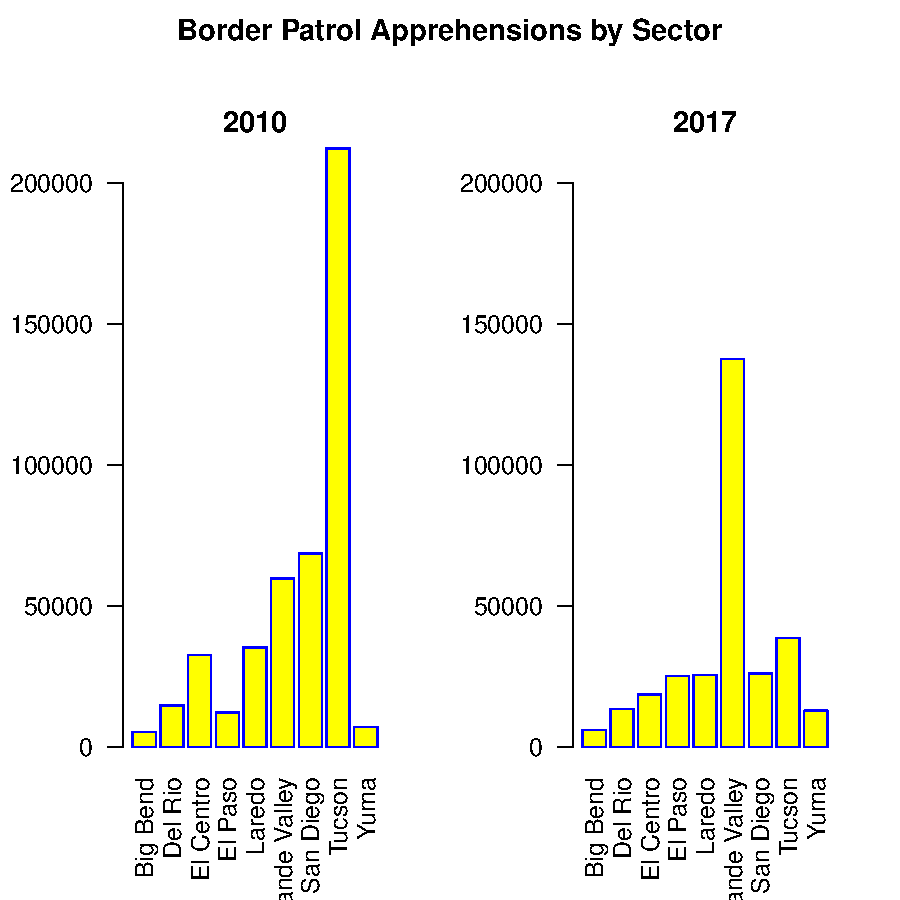
\includegraphics{Document-003}

\subsection{By Sector (Way Two)}

\begin{Schunk}
\begin{Sinput}
> year2010 <- t(as.data.frame(matrix(A2010[1:9,13])))
> colnames(year2010) <- rownames(A2010[1:9,])
> year2017 <- t(as.data.frame(matrix(A2017[1:9,13])))
> colnames(year2017) <- rownames(A2017[1:9,])
> year2010_17 <- rbind(year2010, year2017)
> row.names(year2010_17) <- c("2010", "2017")
> barplot(as.matrix(year2010_17), beside = TRUE, col = c("red", "blue"), bty="n",las=2)
> legend("topleft", c("2010","2017"), pch=15,  col=c("red","blue"),  bty="n")
> title("Border Patrol Apprehensions by Sector")
\end{Sinput}
\end{Schunk}
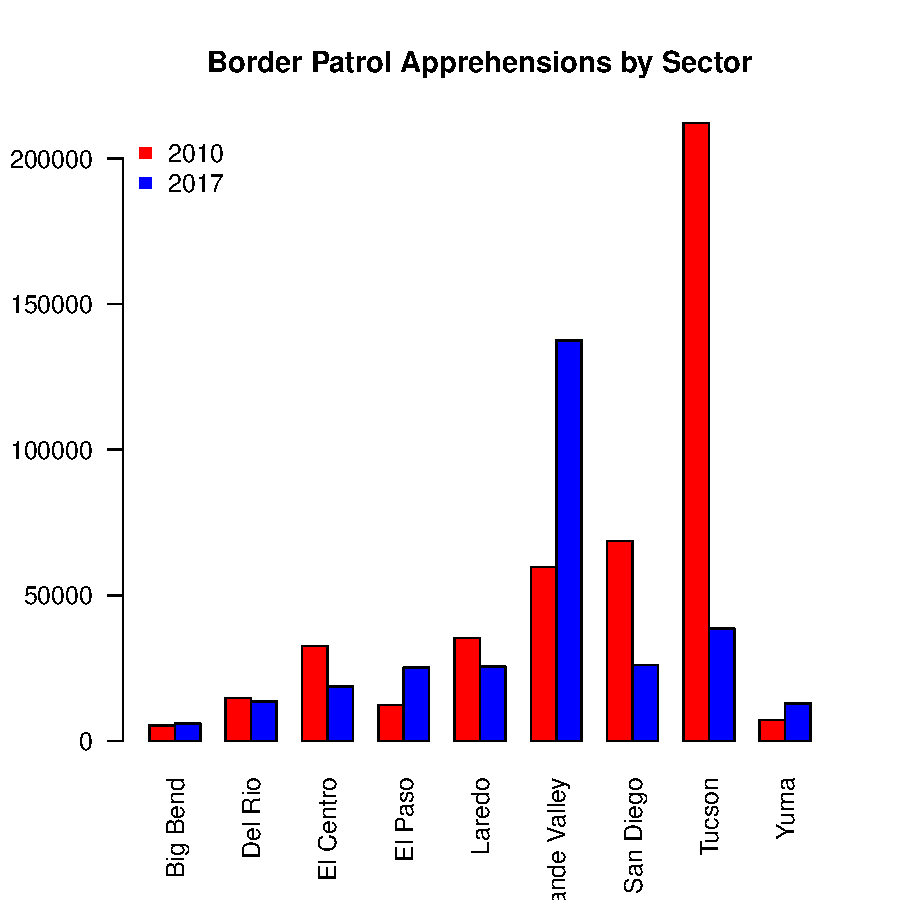
\includegraphics{Document-004}
    
\subsection{By Month}
\begin{Schunk}
\begin{Sinput}
> par(mfcol=c(1,2),oma=c(0,0,2,0))
> barplot(unname(t(A2010)[1:12,10]), 
+         names.arg = colnames(A2010)[1:12], 
+         las=2,
+         axisnames=TRUE,
+         main="2010",
+         border="blue",
+         col="yellow",
+         ylim=c(0,60000))
> barplot(unname(t(A2017)[1:12,10]), 
+         names.arg = colnames(A2017)[1:12], 
+         las=2,
+         axisnames=TRUE,
+         main="2017",
+         border="blue",
+         col="yellow",
+         ylim=c(0,60000))
> title("Border Patrol Apprehensions by Month", outer=TRUE)
\end{Sinput}
\end{Schunk}
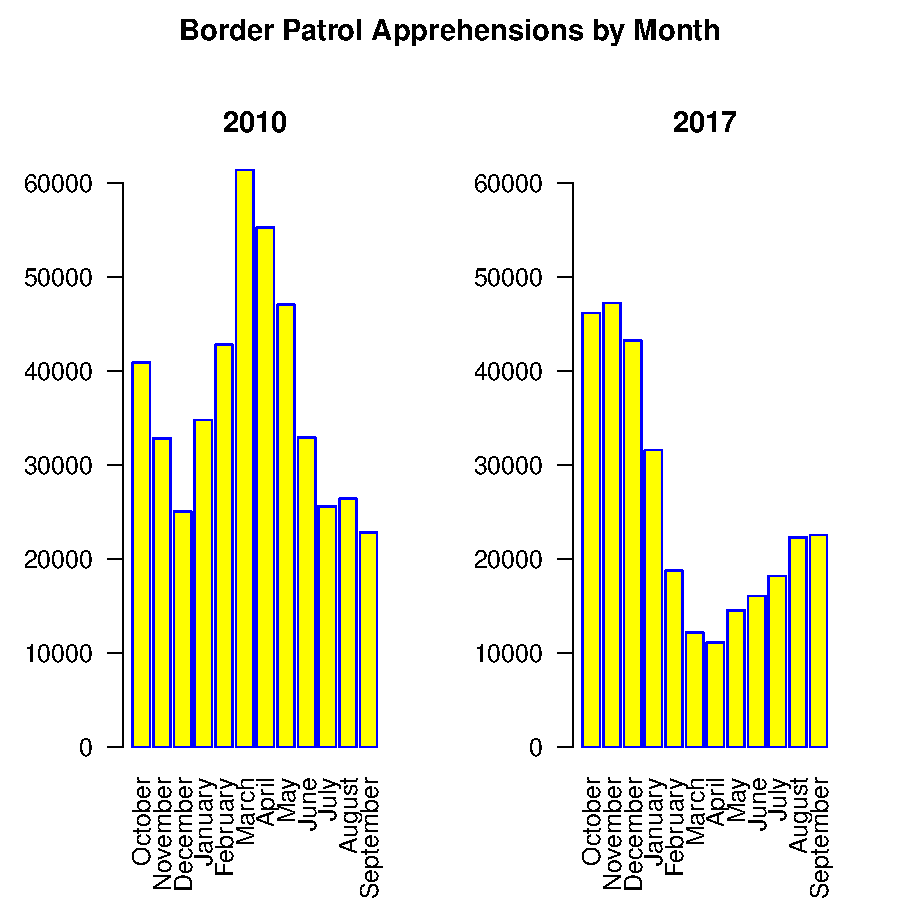
\includegraphics{Document-005}

\subsection{t-test}

\subsubsection{Comparison between sector with most apprehensions for 2010 with sector with most apprehensions in 2017}

\begin{Schunk}
\begin{Sinput}
> Sector_Totals_2010 <- A2010[1:9,13]
> names(Sector_Totals_2010) <- rownames(A2010[1:9,])
> Sector_Totals_2017 <- A2017[1:9,13]
> names(Sector_Totals_2017) <- rownames(A2017[1:9,])
> MA_2017_index <- which(Sector_Totals_2017 == max(Sector_Totals_2017))
> MA_2010_index <- which(Sector_Totals_2010 == max(Sector_Totals_2010))
> MA_2017 <- A2017[MA_2017_index,1:12]
> MA_2010 <- A2010[MA_2010_index,1:12]
> t.test(MA_2010,MA_2017)
\end{Sinput}
\begin{Soutput}
	Welch Two Sample t-test

data:  MA_2010 and MA_2017
t = 1.9547, df = 21.973, p-value = 0.06346
alternative hypothesis: true difference in means is not equal to 0
95 percent confidence interval:
  -379.5935 12819.5935
sample estimates:
mean of x mean of y 
  17683.5   11463.5 
\end{Soutput}
\begin{Sinput}
> t.test(MA_2010,A2017[MA_2010_index,1:12])
\end{Sinput}
\begin{Soutput}
	Welch Two Sample t-test

data:  MA_2010 and A2017[MA_2010_index, 1:12]
t = 6.4303, df = 11.781, p-value = 3.545e-05
alternative hypothesis: true difference in means is not equal to 0
95 percent confidence interval:
  9551.716 19372.450
sample estimates:
mean of x mean of y 
17683.500  3221.417 
\end{Soutput}
\begin{Sinput}
> t.test(MA_2017,A2010[MA_2017_index,1:12])
\end{Sinput}
\begin{Soutput}
	Welch Two Sample t-test

data:  MA_2017 and A2010[MA_2017_index, 1:12]
t = 2.7789, df = 11.846, p-value = 0.01686
alternative hypothesis: true difference in means is not equal to 0
95 percent confidence interval:
  1392.65 11573.35
sample estimates:
mean of x mean of y 
  11463.5    4980.5 
\end{Soutput}
\end{Schunk}

\subsubsection{compare 3 month periods with the most apprehensions in 2010 and 2017}

\begin{Schunk}
\begin{Sinput}
> col <- c("Oct-Dec", "Jan-Mar", "Apr-Jun","Jul-Sep")
> Monthly_Totals_2010 <- (t(A2010)[1:12,10])
>   #Breakdown 
>   A2010_3 <- rbind(sum(Monthly_Totals_2010[1:3]),sum(Monthly_Totals_2010[4:6]),sum(Monthly_Totals_2010[7:9]),sum(Monthly_Totals_2010[10:12]))
> Monthly_Totals_2017 <- (t(A2017)[1:12,10])
>   #Breakdown 
>   A2017_3 <- rbind(sum(Monthly_Totals_2017[1:3]),sum(Monthly_Totals_2017[4:6]),sum(Monthly_Totals_2017[7:9]),sum(Monthly_Totals_2017[10:12]))
> t.test(Monthly_Totals_2010[4:6],Monthly_Totals_2017[1:3])
\end{Sinput}
\begin{Soutput}
	Welch Two Sample t-test

data:  Monthly_Totals_2010[4:6] and Monthly_Totals_2017[1:3]
t = 0.095848, df = 2.0908, p-value = 0.932
alternative hypothesis: true difference in means is not equal to 0
95 percent confidence interval:
 -32101.2  33627.2
sample estimates:
mean of x mean of y 
 46311.67  45548.67 
\end{Soutput}
\end{Schunk}

\section{Overall Trends}

\subsection{Data Cleaning}
\begin{Schunk}
\begin{Sinput}
> A2000.2017 <- read.csv("PB monthly summaries.csv", header = TRUE, stringsAsFactors = FALSE)
> ## Use strings in Col 1 as row names
> rownames(A2000.2017) <- A2000.2017[,1]
> ## Drop column 1
> A2000.2017 <-  subset(A2000.2017, select= -c(year))
> ## Reorder
> A2000.2017 <- A2000.2017[18:1,]
> rownames(A2000.2017) <- c()
> A2000.2017 <- unname(A2000.2017)
\end{Sinput}
\end{Schunk}

\subsection{Time Series}
\begin{Schunk}
\begin{Sinput}
> ts2 <- as.vector(t(A2000.2017))
> time_series <- ts(ts2, start = c(2000,10), frequency=12)
> ts.plot(time_series, gpars=list(xlab="year", ylab="Apprehensions", lty=c(1:3)))
> meanbyyear <- rowMeans(A2000.2017)
> years <- c(2000:2017)
> lines(years,meanbyyear,col="red")
> title("Border Patrol Apprehensions Year")
> legend("topright", c("Average Apprehensions"), pch=15,  col="red",  bty="n")
\end{Sinput}
\end{Schunk}
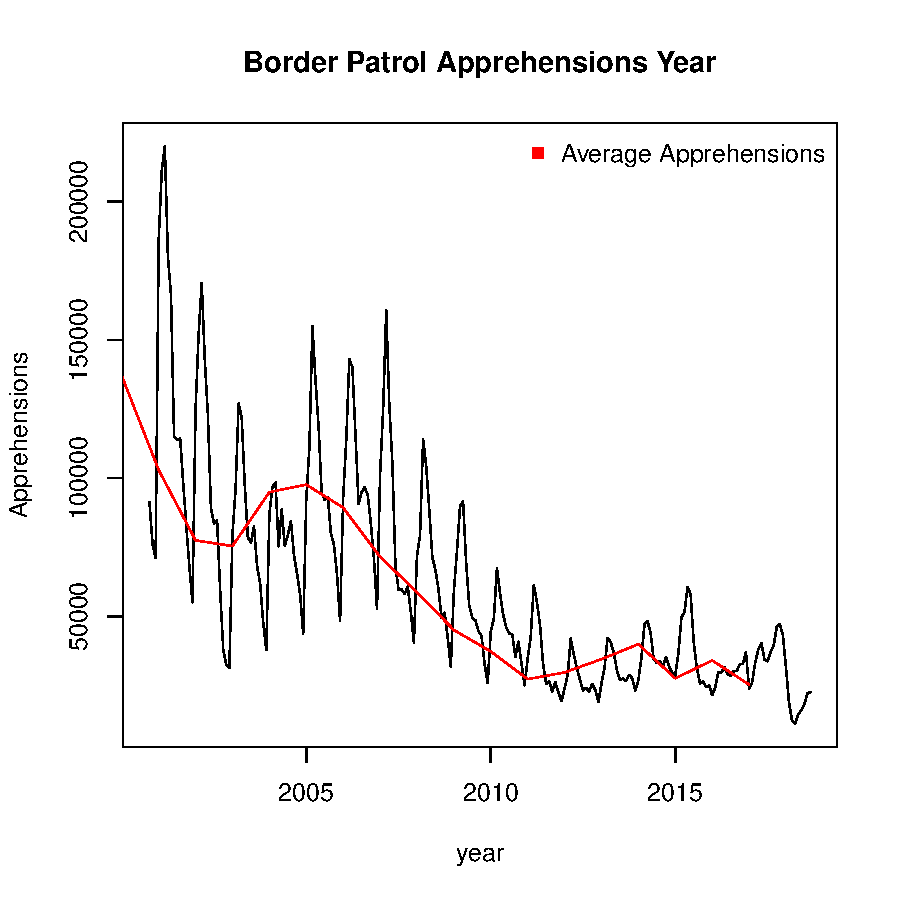
\includegraphics{Document-009}

\end{document}
